\section{Clasificación de columnas atómicas e identificación de estructuras por IA}

La filosofía de los algoritmos de ML (Machine Learning) es que los programas sean capaces de realizar tareas para las que no han sido programados. En nuestro caso, nos interesa aprovechar las grandes capacidades que estos modelos presentan para resolver problemas masivos de identificación de estructuras.\\

Una vez hemos logrado localizar y caracterizar nuestras columnas atómicas, ya podemos proceder con su clasificación. Para ello, como generalmente contaremos con una firma en más de 3 dimensiones, recurriremos a métodos basados en inteligencia artificial. En todos ellos, nuestra entrada siempre será la firma de una columna atómica, mientras que la salida corresponderá con su clase.\\

Para entrenar los modelos que exponemos en este trabajo (excepto \textit{K-means}), nos basaremos en el \textbf{aprendizaje supervisado}, de modo que todos los datos de entrenamiento serán previamente analizados y clasificados. No obstante, hay que tener en cuenta que también es posible desarrollar algoritmos basados en aprendizaje no supervisado, semi-supervisado o reforzado.\\

\subsection{Métodos para análisis de \textit{clusters}}
El análisis de \textit{clusters} es un método estadístico de procesamiento de datos. Su función principal consiste en organizar los distintos elementos de un \textit{dataset} en grupos, teniendo en cuenta su distancia dentro del espacio que generan las variables de entrada.\\

\begin{figure}[h!]
    \centering
    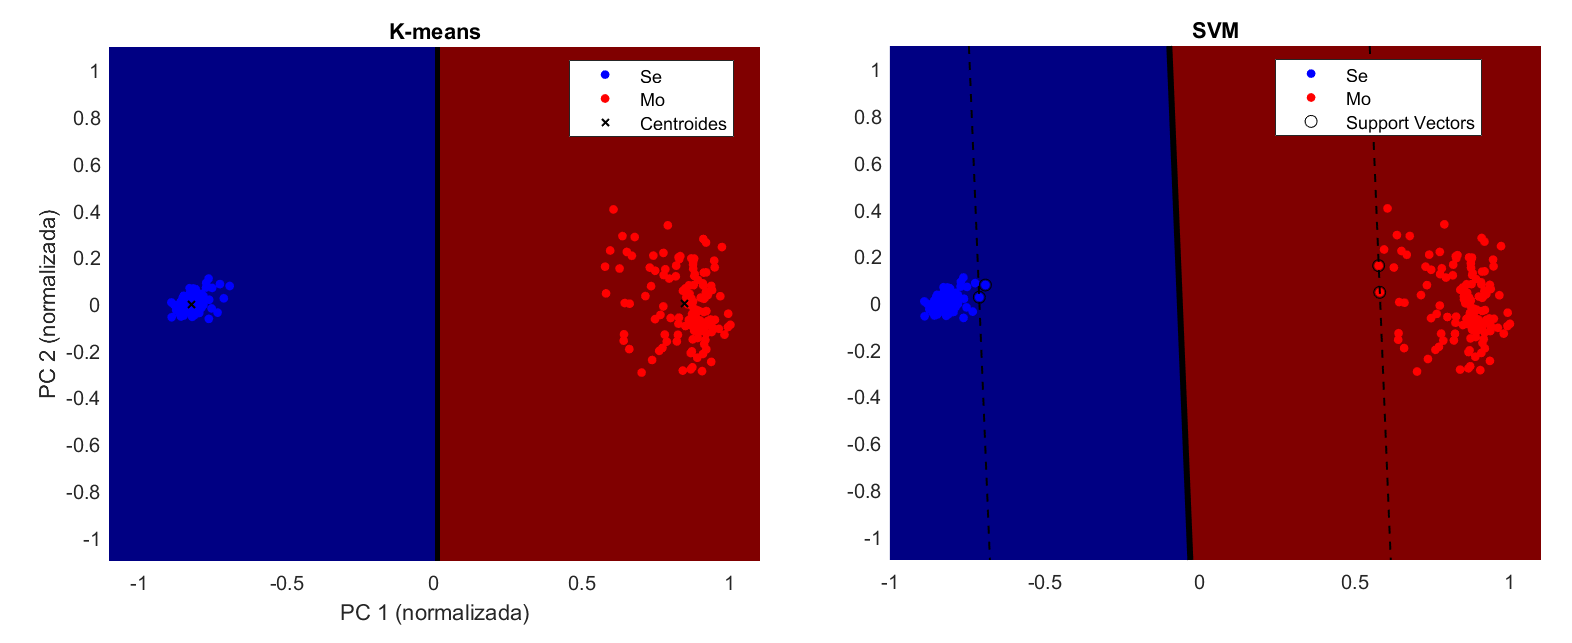
\includegraphics[width=1\textwidth]{fig/Fig12.png}
    \caption{Clasificación realizada por \textit{K-means} ($k=2$) y SVM para el caso de la \autoref{fig:9}. Se muestra la recta que separa las distintas regiones, los centroides de \textit{K-means} y el margen entre clases del SVM. Para ajustar estos modelos se han aprovechado las funciones \textit{fitcsvm} y \textit{kmeans} contenidas en el paquete \textit{Statistics and Machine Learning Toolbox} de MATLAB \cite{repo}.}
    \label{fig:12}
\end{figure}

\subsubsection{\textit{Support Vector Machine} (SVM)}
SVM es un algoritmo de aprendizaje supervisado que permite encontrar el hiperplano que mejor separa dos \textit{clusters} de datos distintos. Tal y como se observa en la \autoref{fig:12}, el método se encarga de maximizar el margen entre clases, que corresponde con la anchura máxima de la región paralela al hiperplano que no contiene puntos de datos.

\subsubsection{\textit{K-means}}
Este algoritmo parte de una serie de observaciones y se encarga de organizarlas en los $k$ grupos que nosotros le indiquemos. Para llevar a cabo esta clasificación sigue un criterio muy simple: Asignar cada medida al \textit{cluster} cuyo valor medio asociado sea el más cercano.\\

Dado que este método es de aprendizaje no supervisado, en vista de los resultados de la \autoref{fig:12}, si entre nuestros datos contáramos con algún tipo de vacante o intersticial, podríamos ajustar $k$ para que dicho tipo de columnas atómicas pertenecieran a otro grupo distinto.

% --
\subsection{\textit{Deep Learning} (DL)}
El DL está contenido por definición dentro de los algoritmos de ML, no obstante, en este caso se hace uso de estructuras más complejas que tratan de simular el cerebro humano, las redes neuronales. Las técnicas de DL que han ganado más protagonismo en el campo de la visión por ordenador son las CNN (\textit{Convolutional Neural Networks}), las RNN (\textit{Recurrent Neural Networks}) y los transformadores.\\

\begin{wrapfigure}{o}{6.5cm}
    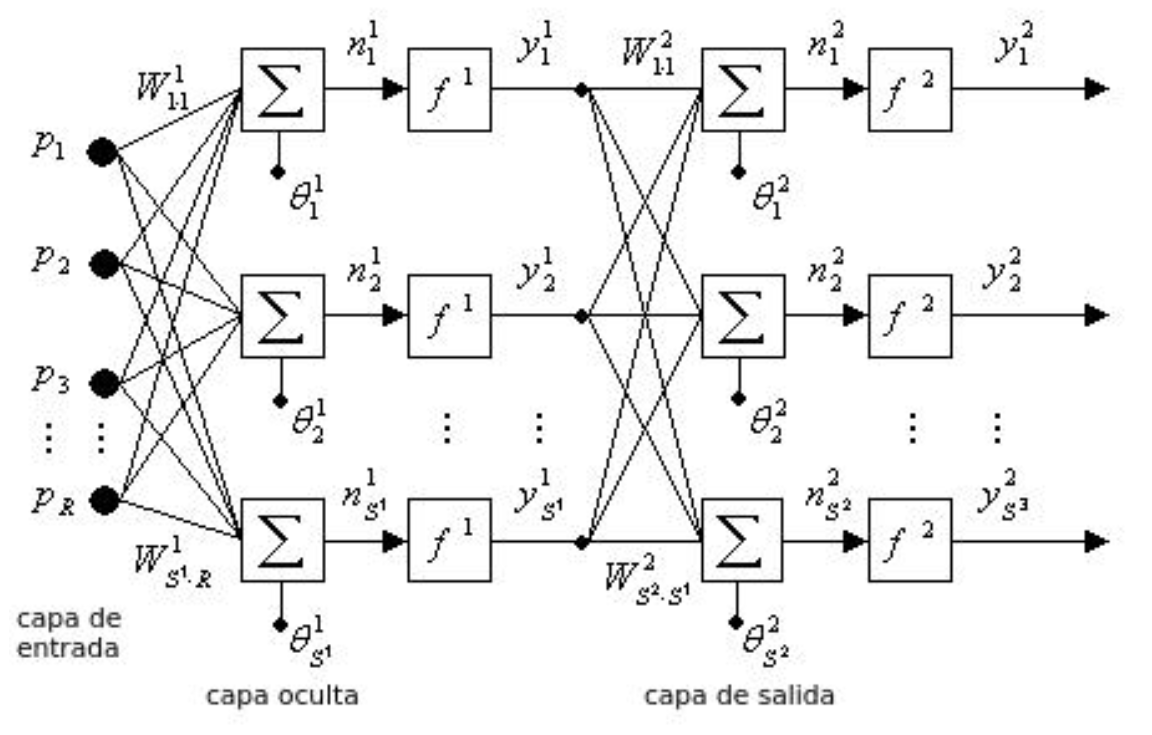
\includegraphics[width=0.40\textwidth]{fig/Fig13.png}
    \caption{Esquema de una red neuronal artificial. Extraído de la referencia \cite{red}.}
    \label{fig:13}
\end{wrapfigure} 

A nivel fundamental, estas redes van a estar compuestas por unas unidades básicas de procesamiento, que llamaremos neuronas, agrupadas por capas. Cada neurona $n_i^l$ contará con una cantidad de entradas $x_j^l$ igual al número de neuronas de la capa anterior, un término independiente $\theta_i^l$ y una función de activación $f^l$. Todas las entradas vendrán pesadas por un parámetro $w_{ij}^l$ que podrá ser modulado durante el entrenamiento (ver \autoref{fig:13}).\\

Cuando la red realiza un \textit{forward pass}, cada neurona de la capa de inicial toma las distintas variables de entrada, las pesa con su parámetro correspondiente y realiza un sumatorio que posteriormente introduce en la función de activación para suministrar una la salida $y_i^l$. Cada una de estas salidas actúa como entrada para las neuronas de la siguiente capa, y este proceso se repite hasta alcanzar la capa de salida. Lo que se logra así es realizar una serie de transformaciones lineales encadenadas, llevando los datos de entrada a un nuevo espacio desde el cuál poder clasificarlos (algo similar a lo que hicimos con el PCA).\\

\newpage
Para entrenar a la red se realiza un \textit{backward pass}, computando el error $\delta_i^L $ de la última capa mediante una función de coste (que depende de $y_i^L$ y $z_i$, las salidas que esperamos) y propagándolo hacía atrás para determinar el del resto de capas. Posteriormente se aplica un descenso del gradiente que trata de minimizar cada error $\delta_i^l$ modulando los parámetros asociados a la capa $l$, incluidos los independientes.\\

\begin{figure}[h!]
    \centering
    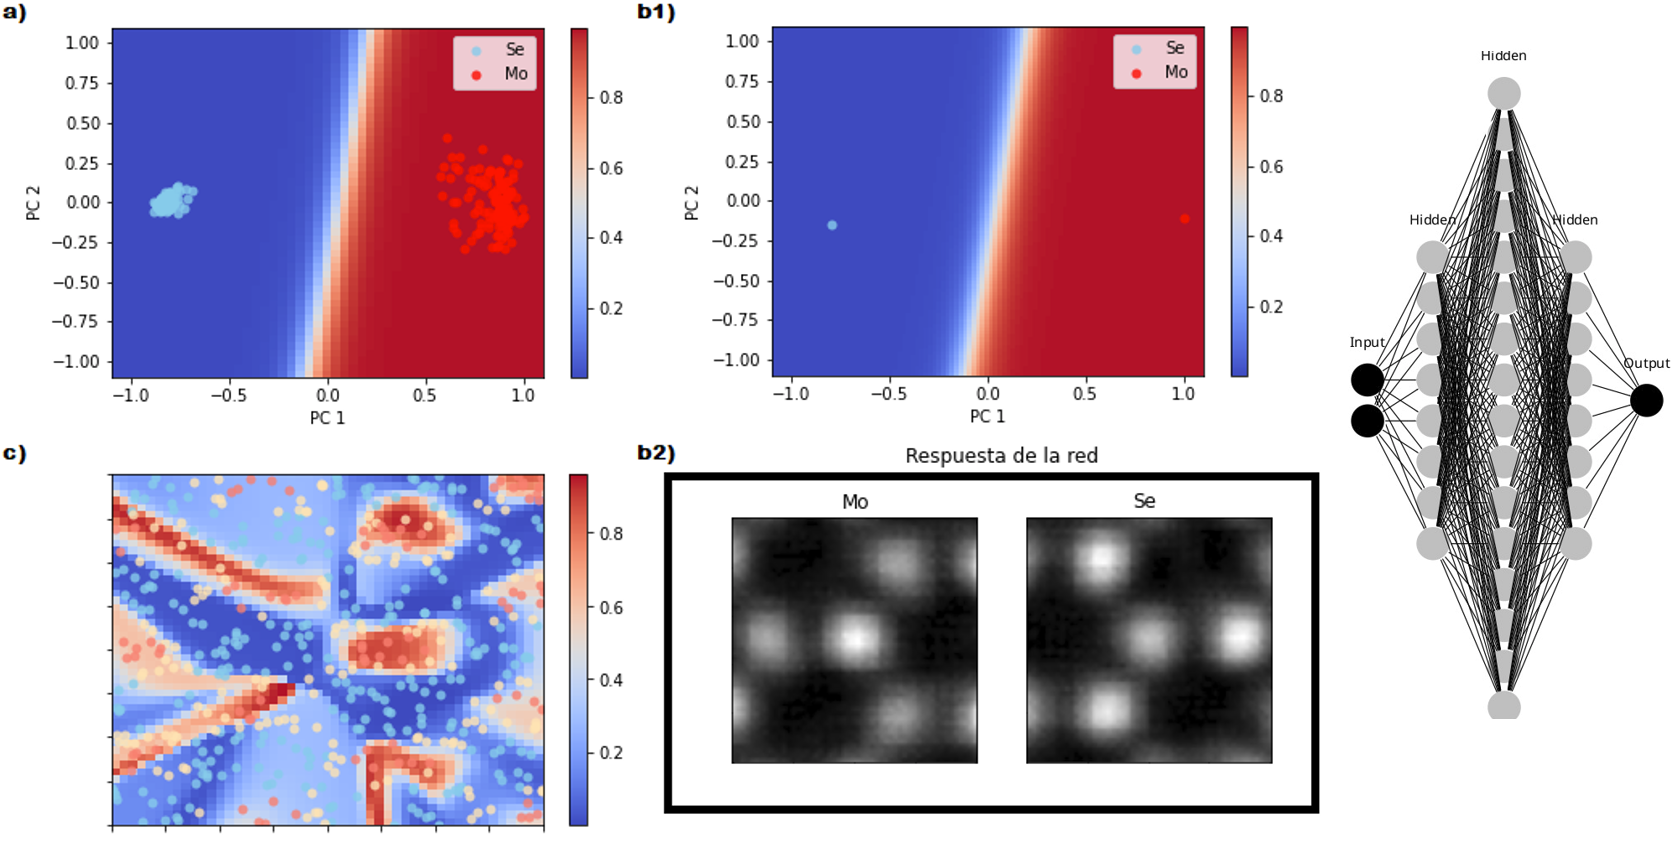
\includegraphics[width=1\textwidth]{fig/Fig14.png}
    \caption{Se muestra \textbf{a)} el conjunto de entrenamiento (tomados de la \ref{fig:9}) y el estado final de la red tras diez mil iteraciones, \textbf{b)} una predicción de la red para dos nuevas entradas, y \textbf{c)} el caso de una red entrenada con un \textit{dataset} mucho más complejo. A la derecha tenemos un esquema de la topología de la red. Programa desarrollado en Python por el autor \cite{repo}.}
    \label{fig:14}
\end{figure}

En las Figuras \ref{fig:14}a y \ref{fig:14}b se recurre a una red neuronal con topología 2-8-16-8-1, de la que se obtienen unos resultados bastante satisfactorios. En el caso concreto de nuestro \textit{dataset}, donde contamos con unos \textit{clusters} perfectamente diferenciados en 2D, realmente no es lo más eficiente recurrir a un algoritmo tan pesado en términos de cálculo. Las técnicas de DL están más enfocadas a situaciones con una complejidad similar, o incluso mucho mayor, a la del caso de la Figura \ref{fig:14}c.\\

Es más, diseñando una red neuronal con la topología adecuada y contando con la potencia de cálculo suficiente, podríamos habernos olvidado de realizar una reducción de dimensionalidad PCA, introduciendo directamente como entrada a la red las observaciones de la matriz $X$. En el siguiente capítulo se mostrará algún ejemplo.
